\setcounter{figure}{0}
\renewcommand{\thefigure}{E.\arabic{figure}}
\renewcommand{\theHfigure}{E.\arabic{figure}}

Este anexo reúne, a mayor tamaño, las vistas de la interfaz web descrita en la
Subsección~\ref{subsec:web_panel_ros2}: los controles de teleoperación y
configuración, la supervisión conjunta de los 18 servomotores y el acceso a los
registros internos de cada AX-12A.

\begin{figure}[H]
    \centering
    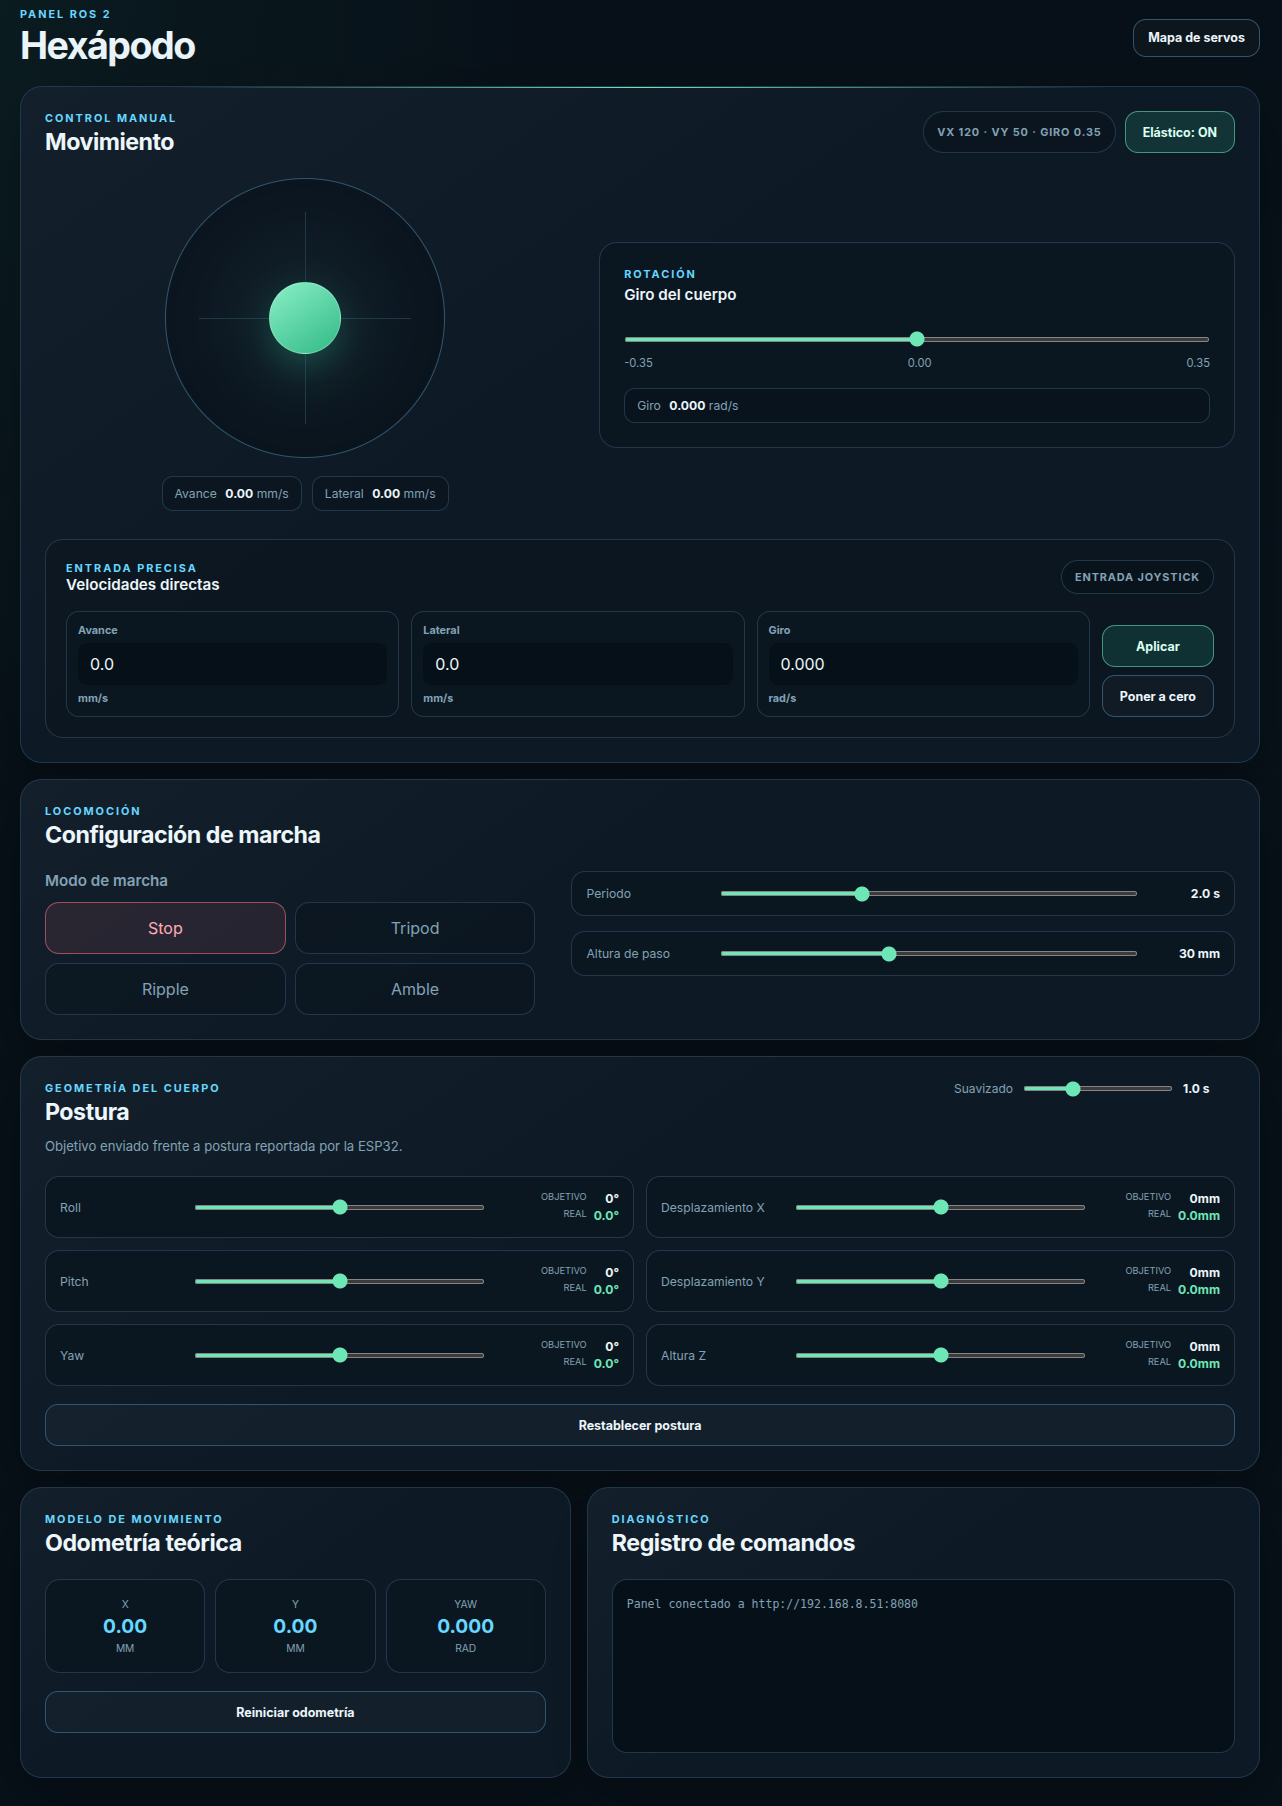
\includegraphics[
        width=0.72\textwidth,
        height=0.62\textheight,
        keepaspectratio
    ]{capitulos/anexos/figuras/panel_web_general.png}
    \captionsetup{justification=centering,singlelinecheck=false}
    \caption[Vista general de la interfaz web]
    {Controles de movimiento, configuración de la marcha, ajuste de la postura y
    odometría estimada.}
    {\centering\footnotesize Fuente: elaboración propia.\par}
    \label{fig:anexo_web_panel_general}
\end{figure}

\clearpage

\begin{figure}[H]
    \centering
    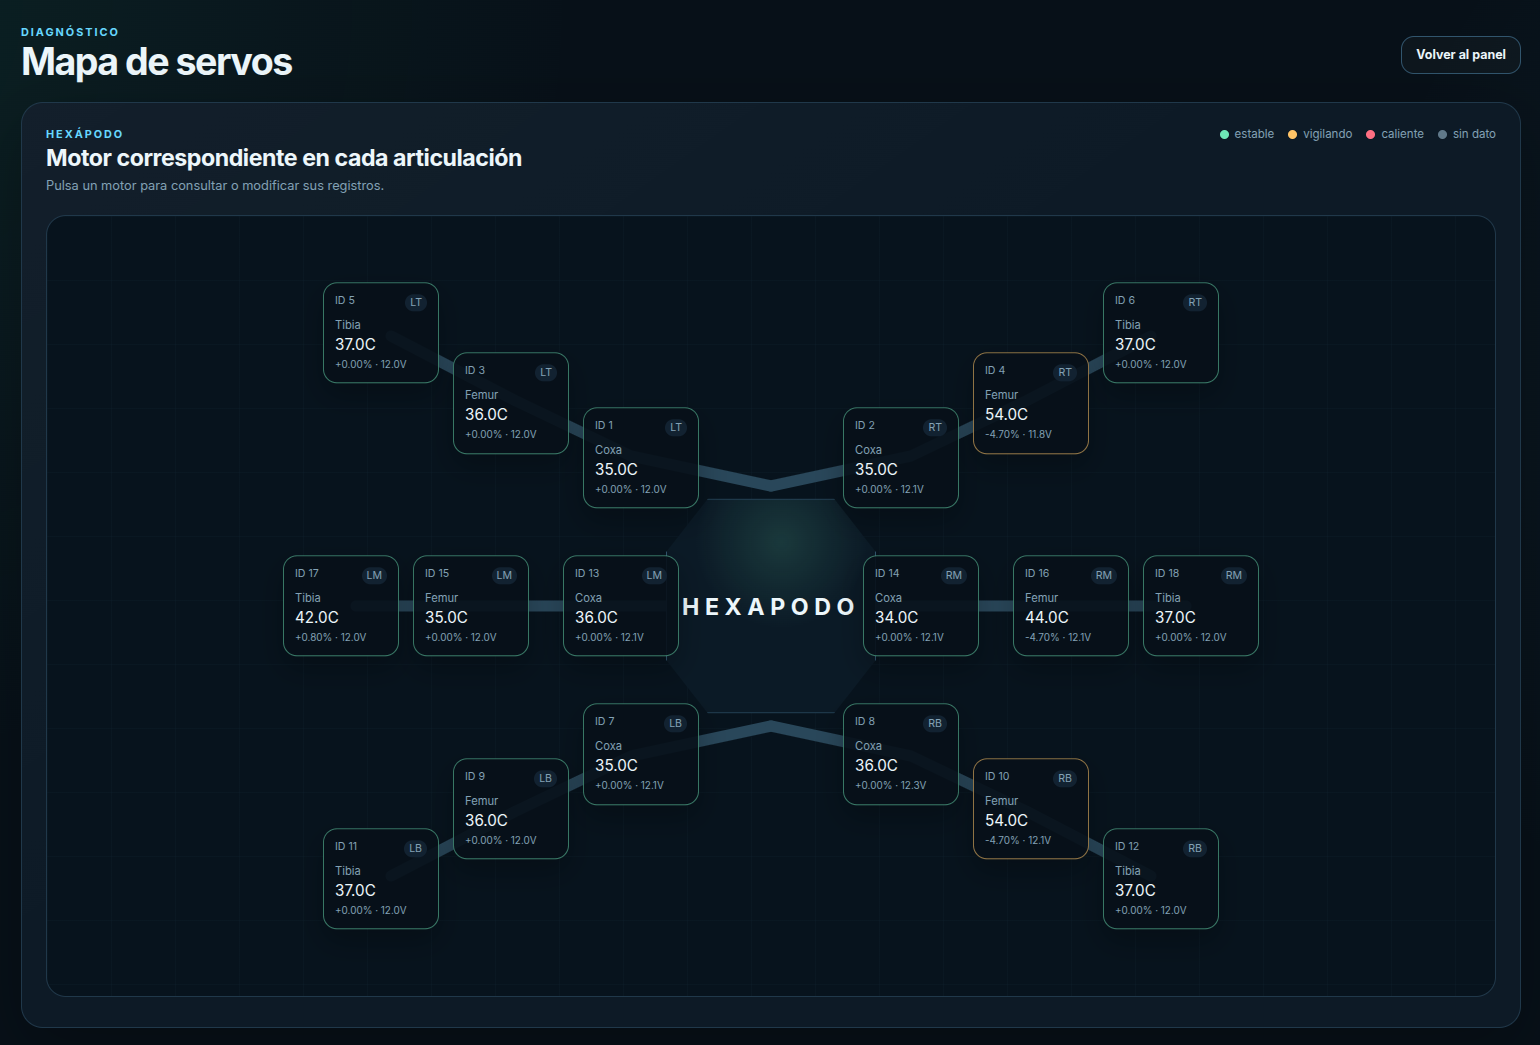
\includegraphics[
        width=0.72\textwidth,
        height=0.34\textheight,
        keepaspectratio
    ]{capitulos/anexos/figuras/panel_web_servos.png}
    \captionsetup{justification=centering,singlelinecheck=false}
    \caption[Mapa de diagnóstico de los servomotores]
    {Distribución de los 18 servomotores con su temperatura, carga y tensión.}
    {\centering\footnotesize Fuente: elaboración propia.\par}
    \label{fig:anexo_web_panel_servos}
\end{figure}

\vspace{-0.2\baselineskip}

\begin{figure}[H]
    \centering
    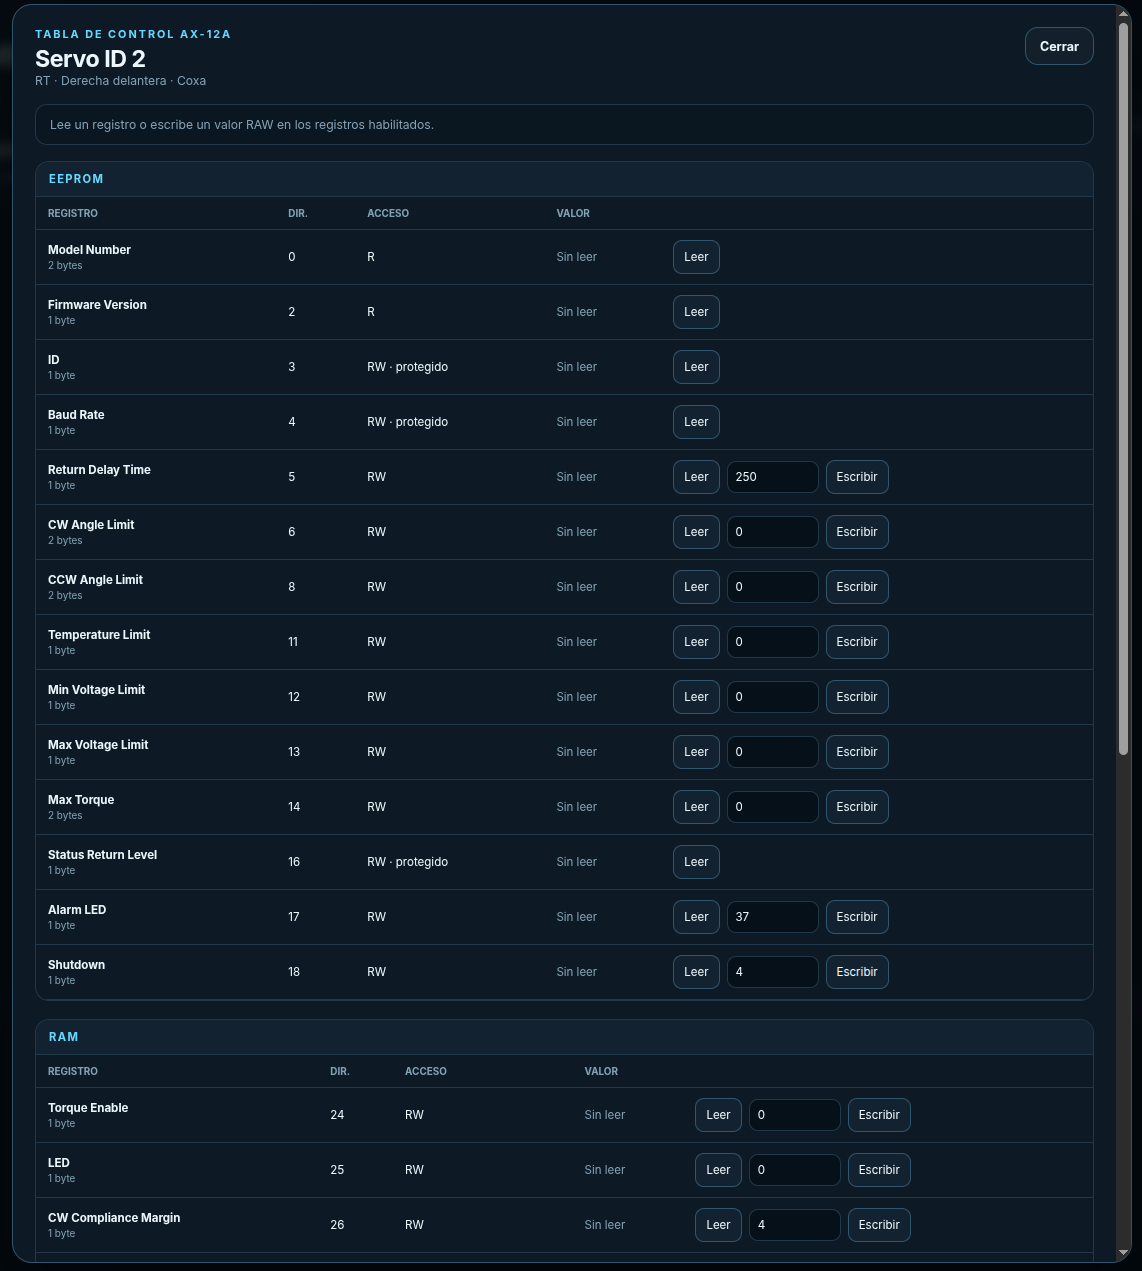
\includegraphics[
        width=0.72\textwidth,
        height=0.54\textheight,
        keepaspectratio
    ]{capitulos/anexos/figuras/panel_web_registros.png}
    \captionsetup{justification=centering,singlelinecheck=false}
    \caption[Acceso a los registros AX-12A]
    {Lectura y escritura de los registros de un servomotor AX-12A.}
    {\centering\footnotesize Fuente: elaboración propia.\par}
    \label{fig:anexo_web_panel_registers}
\end{figure}
